%!TEX root = /Users/stefano/Documents/Bonsai Club/TWBC/twbc.tex

\headline{{\textbf{\Large\sffamily TWBC Workshops:}}\\
          {\textbf{\large\sffamily Carving Bonsai Root Stands}}}
\label{2025-05-rootstands}
\noindent
This month's other workshop was a real treat: Adam guided us through the fascinating world of bonsai \textit{root stands} (\textit{Ne Taku}).  
With his trademark energy and humour, he explained everything from what a root stand is to how you can carve your own --- no fancy equipment required, just creativity, some wood, and a good helping of patience!

Below you'll find the key takeaways from the session: whether you're planning to carve your first stand or just curious about the process, this guide covers everything you need to know.

\medskip
\topic{What Exactly is a Root Stand?}
\noindent
A bonsai root stand (or \textit{Ne Taku} in Japanese) is a free\--form stand with perforations along its sides, crafted from a solid piece of wood. No two are exactly alike --- the shape, colour, and size all depend on the artist's creativity.  
Some stands are small enough to fit in your hand, others can be up to a metre tall!

Root stands pair especially well with \textbf{cascade} or \textbf{semi\--cascade} bonsai styles, where the flowing form of the tree is echoed by the organic, natural shapes of the stand.  
High\--quality examples, especially older or intricately carved ones, can fetch eye\--watering prices on the collector's market.

\medskip
\topic{Getting Started: Materials and Safety First}
\noindent
The journey to a root stand begins with choosing the right piece of wood. Adam recommends using sections of branches or trunks --- or even a solid block --- ideally seasoned (air-dried) for at least a year to help reduce cracking.  
And if the wood has natural features like knots or old branch stubs, even better: these can be incorporated into the design for extra character.

\begin{window}[2,l,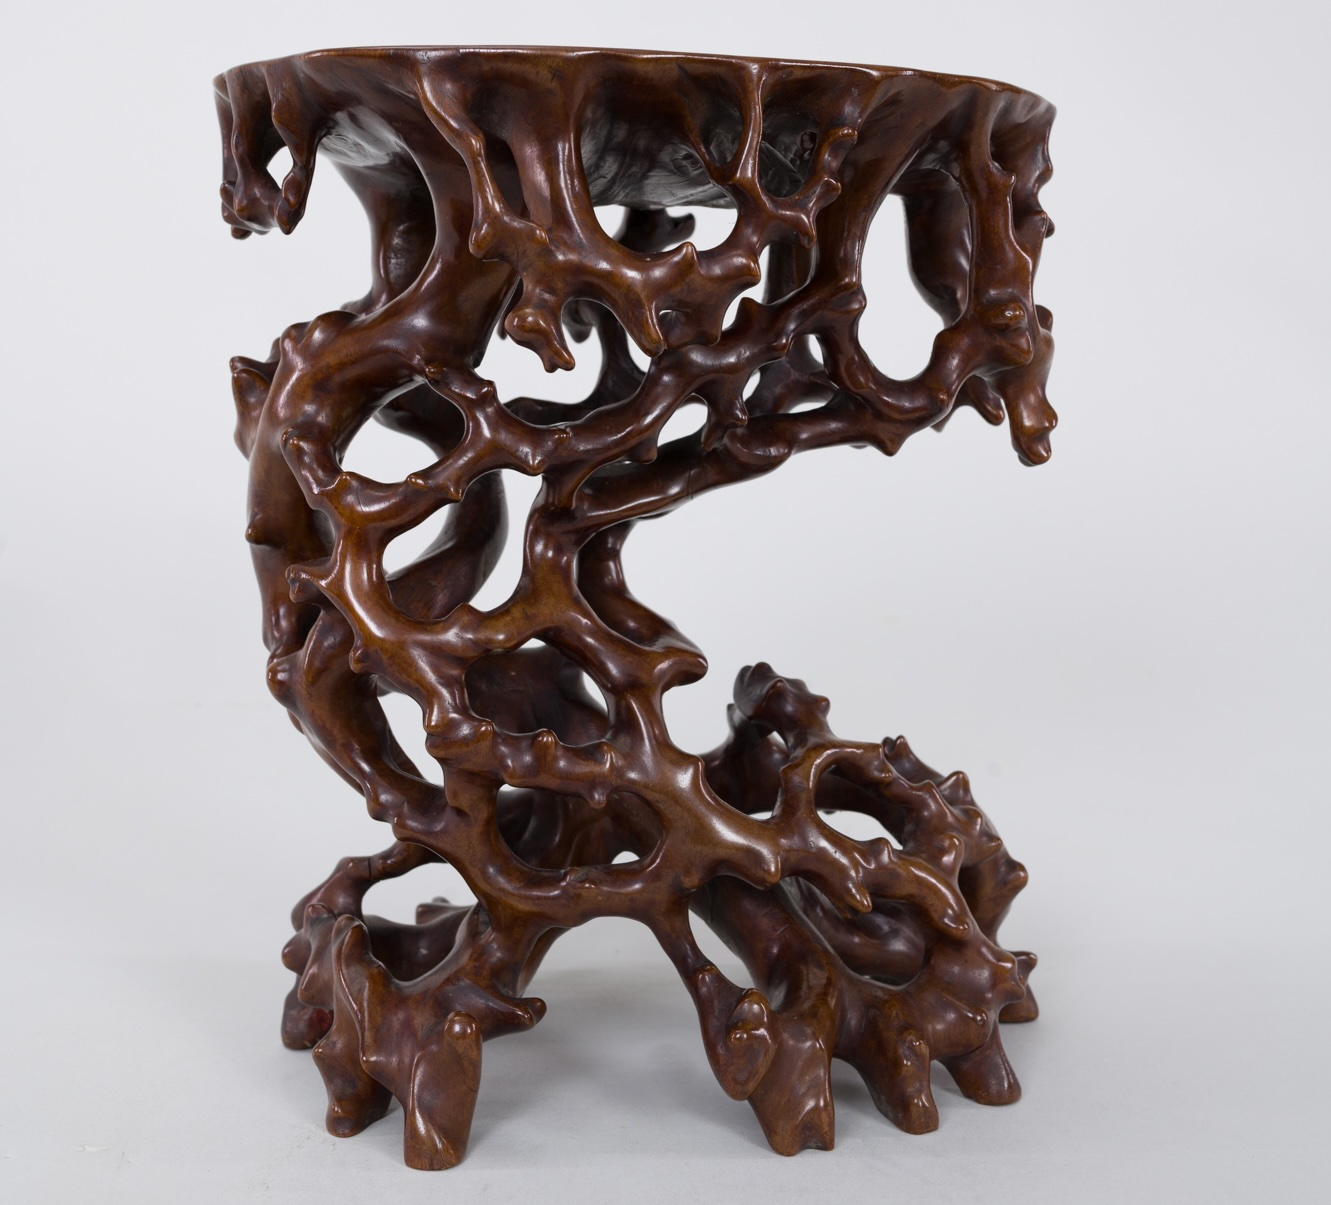
\includegraphics[width=1.0\columnwidth]{2025_05/res/root_stand.jpg},\centerline{\emph{An exquisite example of bonsai root stand.}}]
\end{window}

\begin{figure*}[!t]
\centering
\begin{minipage}[b]{.22\textwidth}
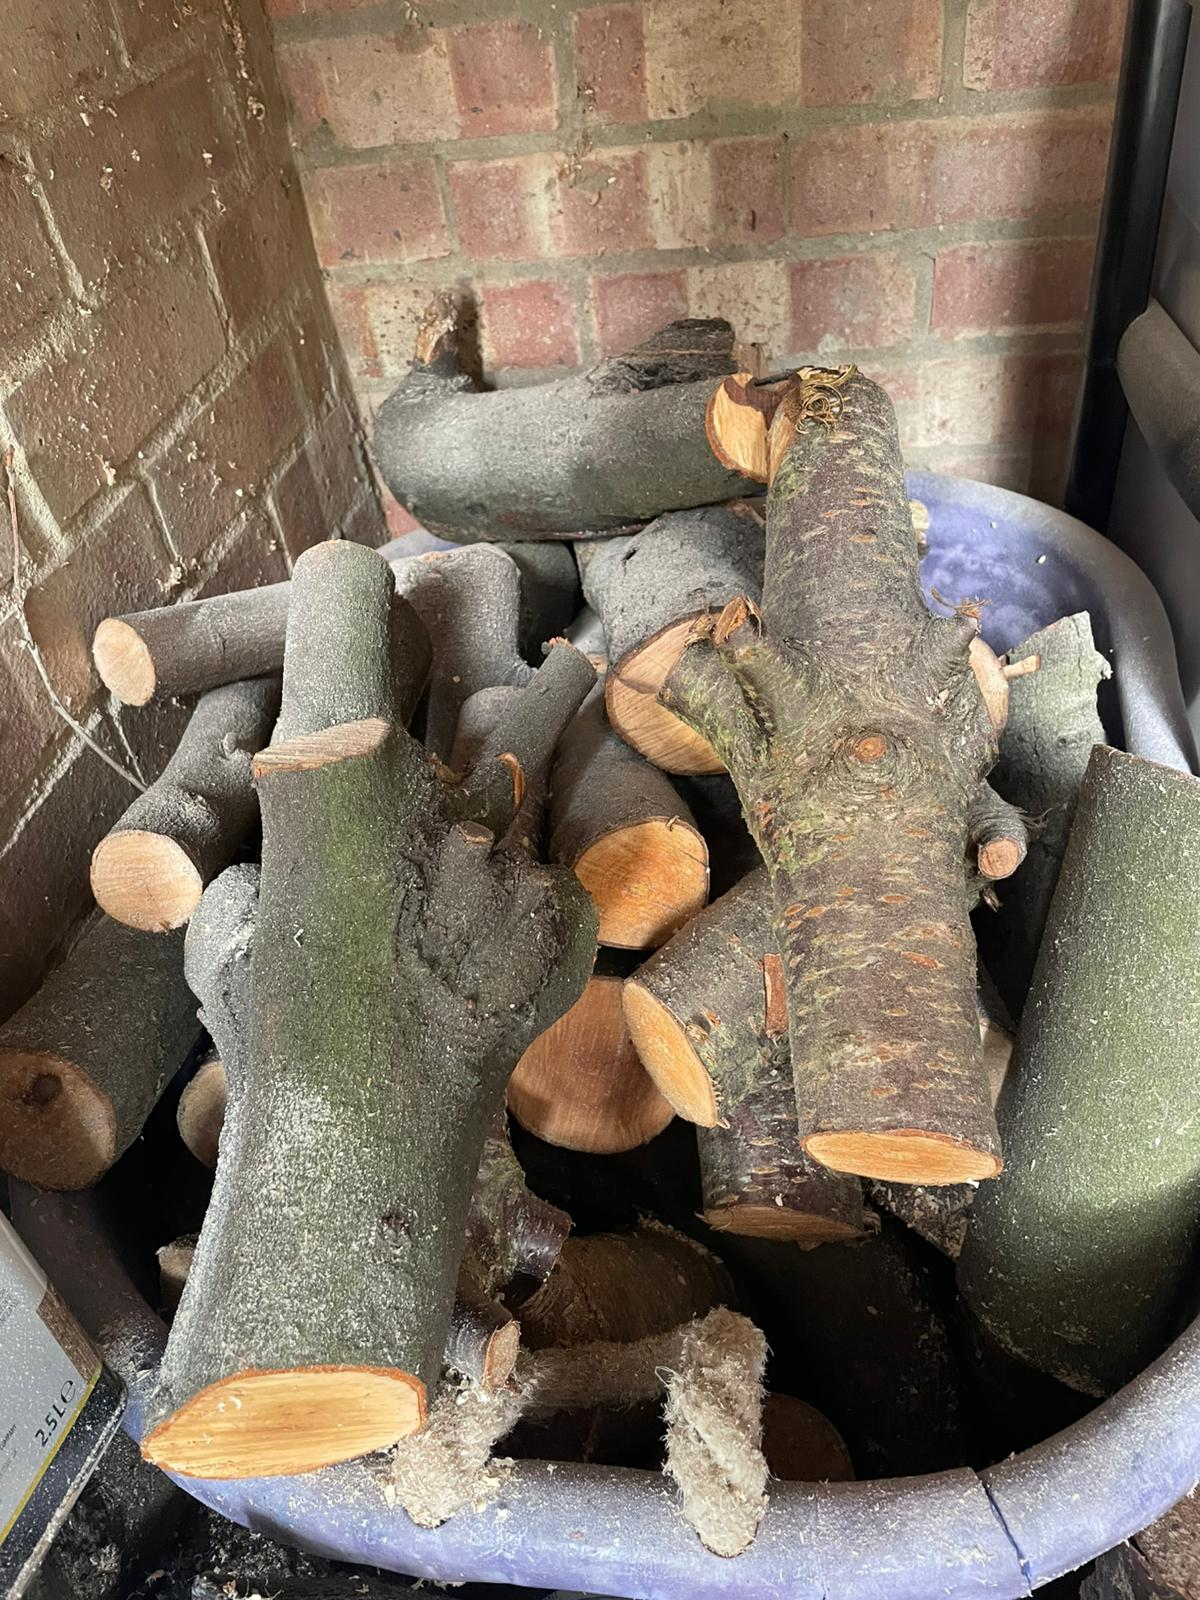
\includegraphics[angle=0,origin=c,width=1.0\textwidth]{2025_05/res/root_stand_stage1.jpeg}
\end{minipage}\qquad
\begin{minipage}[b]{.22\textwidth}
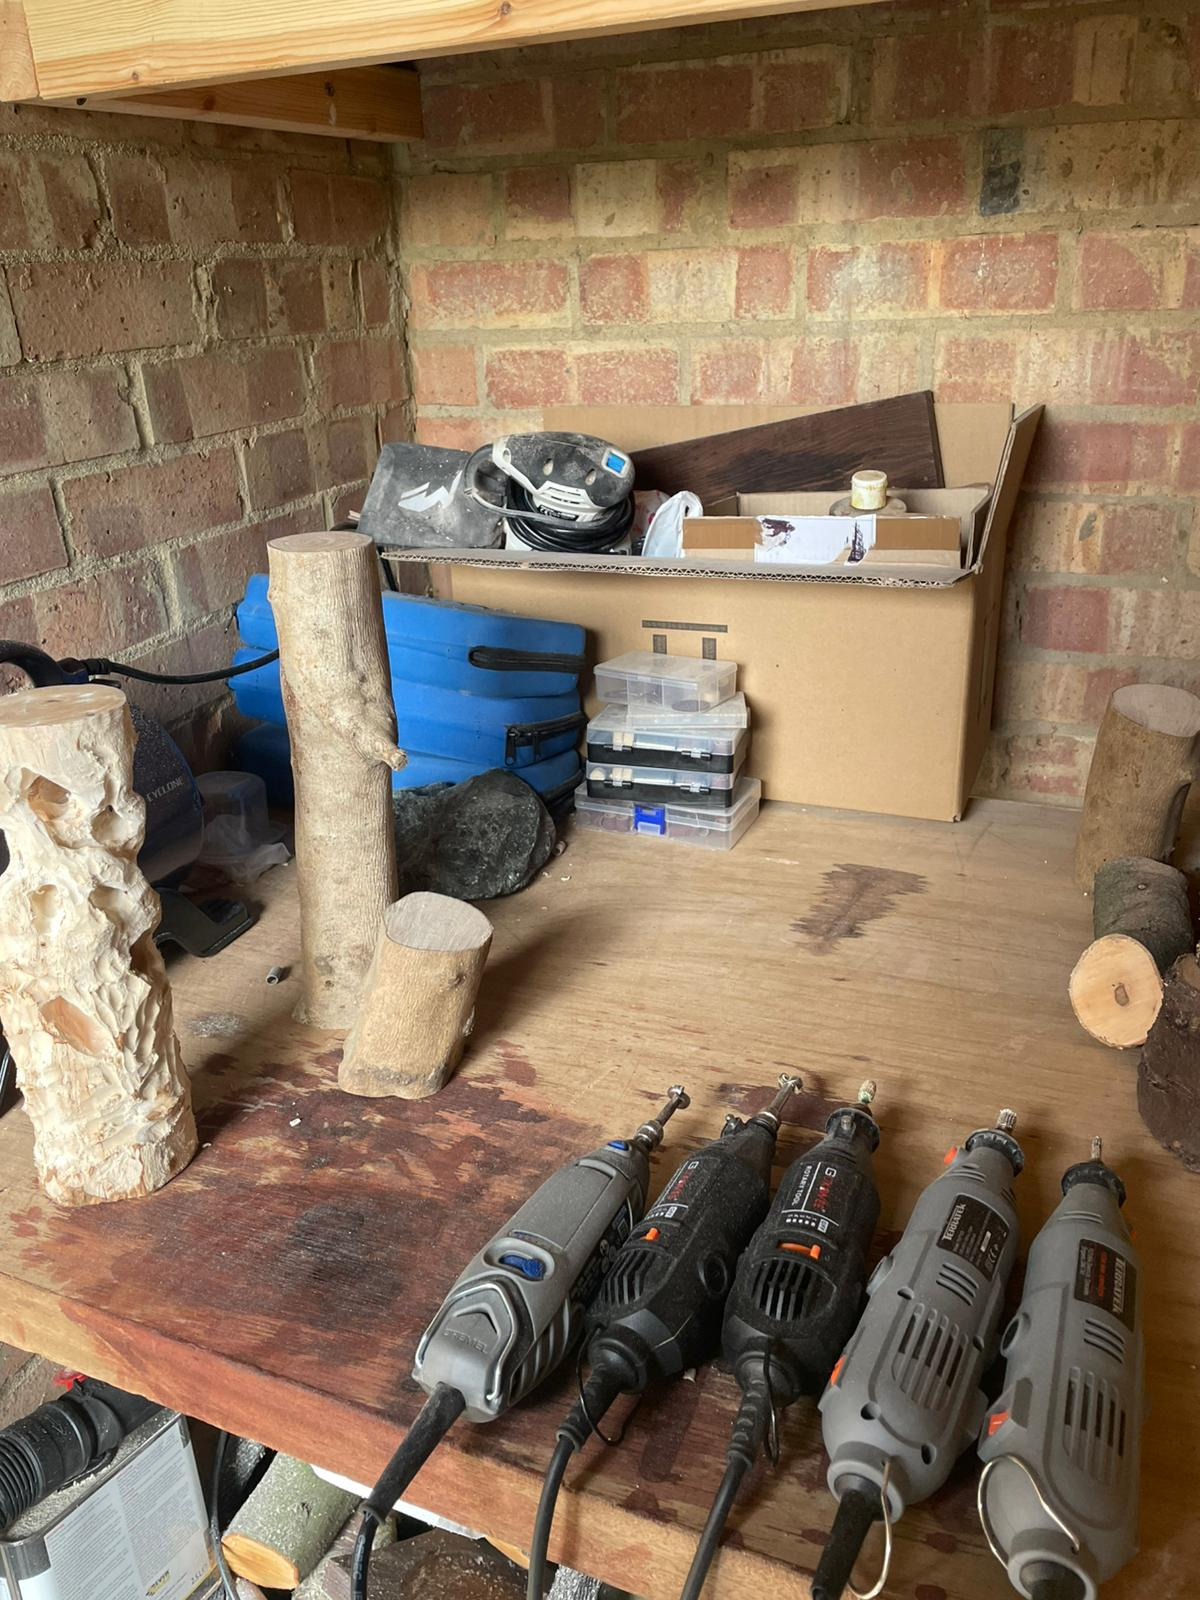
\includegraphics[angle=0,origin=c,width=1.0\textwidth]{2025_05/res/root_stand_stage2.jpeg}
\end{minipage}\qquad
\begin{minipage}[b]{.22\textwidth}
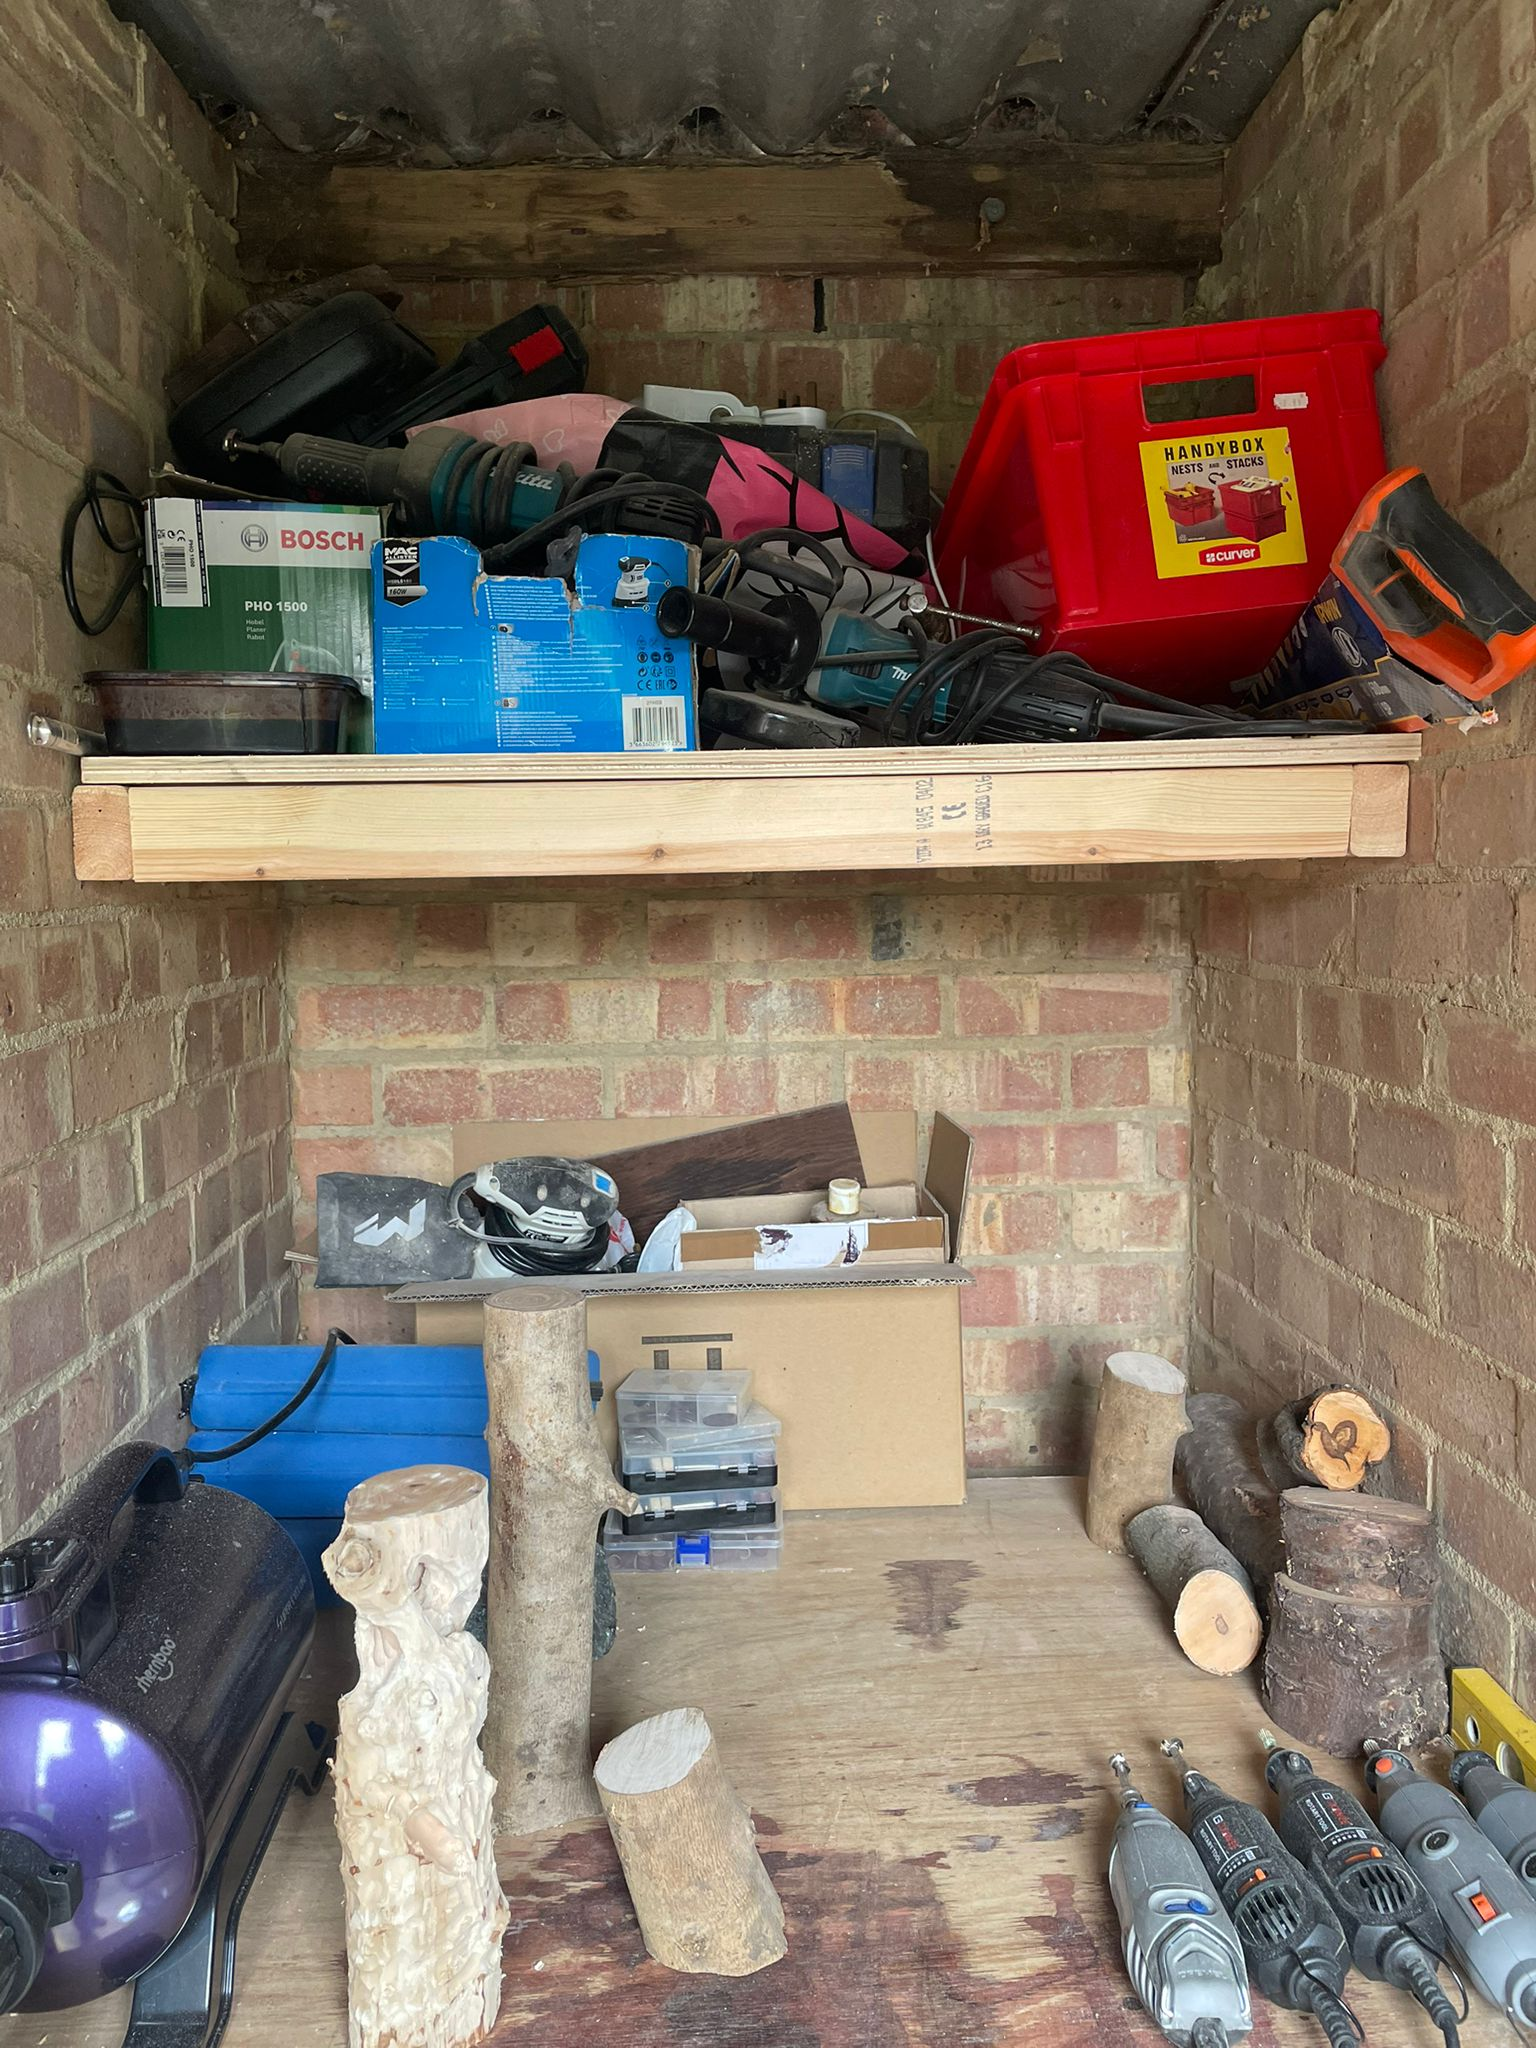
\includegraphics[angle=0,origin=c,width=1.0\textwidth]{2025_05/res/root_stand_stage3.jpeg}
\end{minipage}\qquad
\begin{minipage}[b]{.22\textwidth}
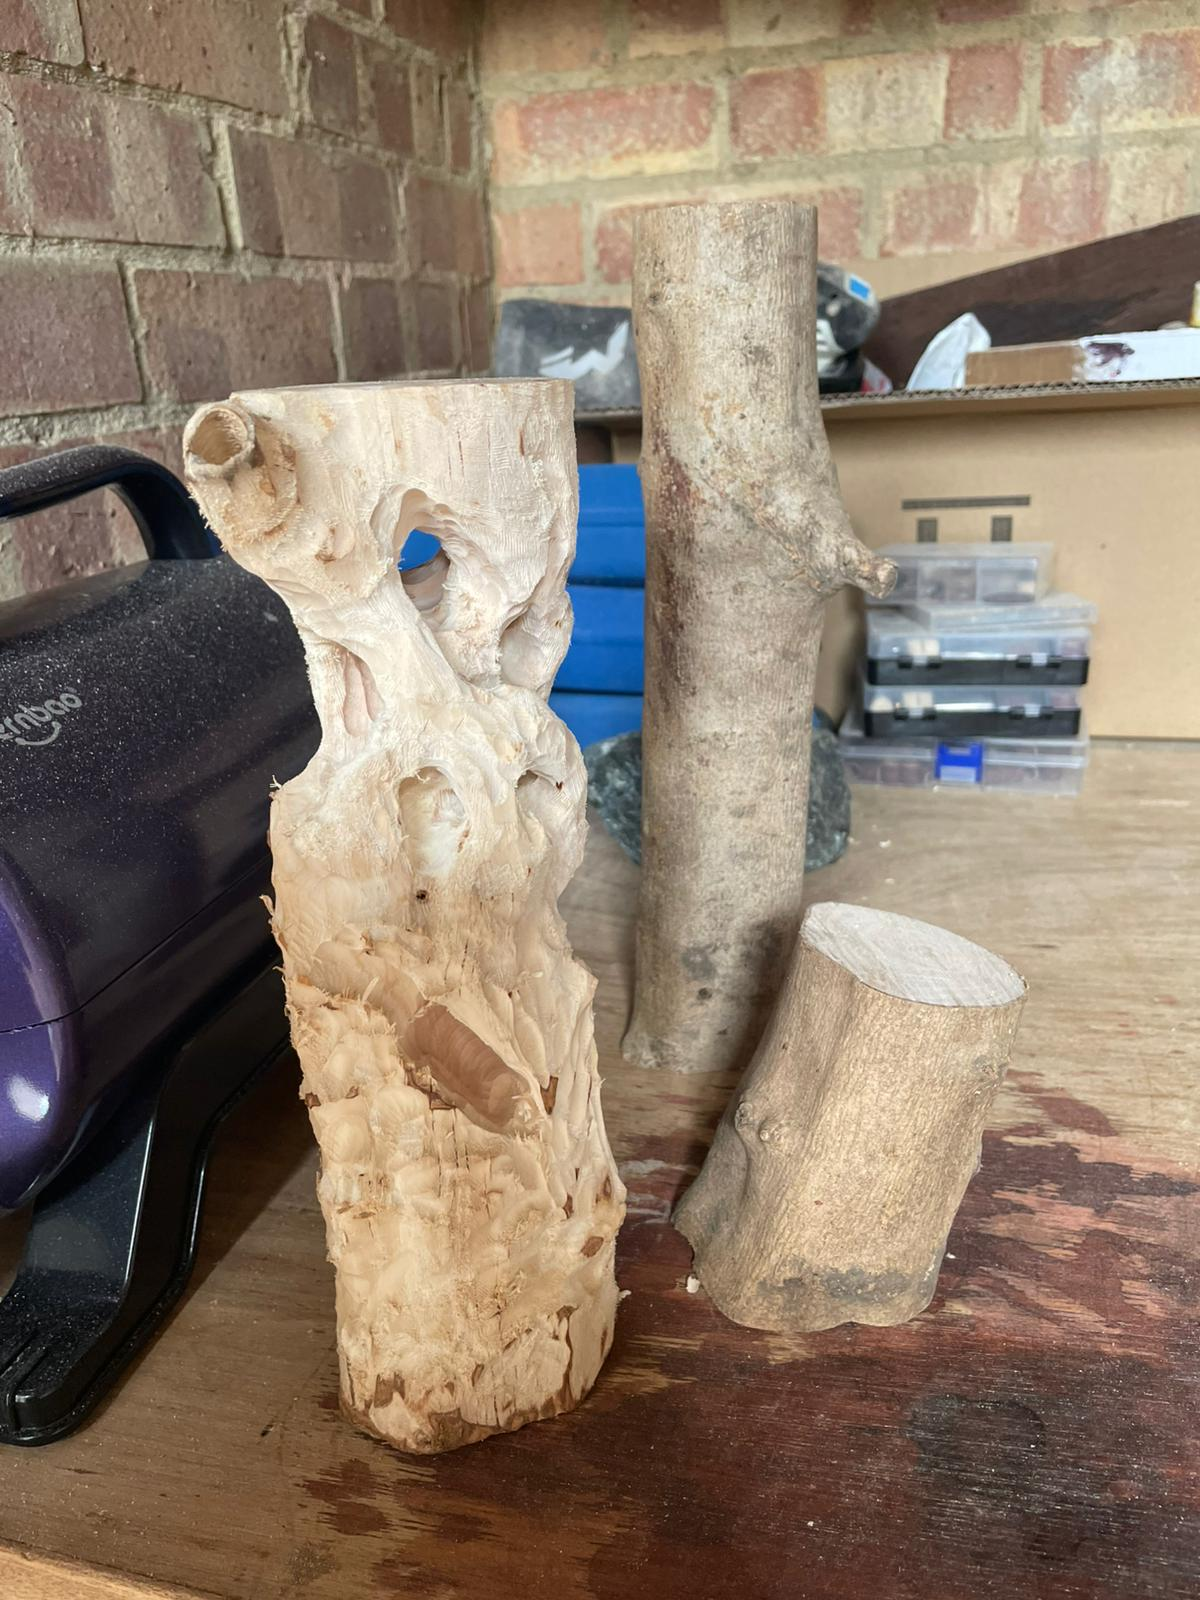
\includegraphics[angle=0,origin=c,width=1.0\textwidth]{2025_05/res/root_stand_stage4.jpeg}
\end{minipage}
\medskip 

\centerline{%
\emph{Adam's ``little shed'' where most of the wood carving magic happens.}}
\end{figure*}

\columnbreak

\begin{window}[2,l,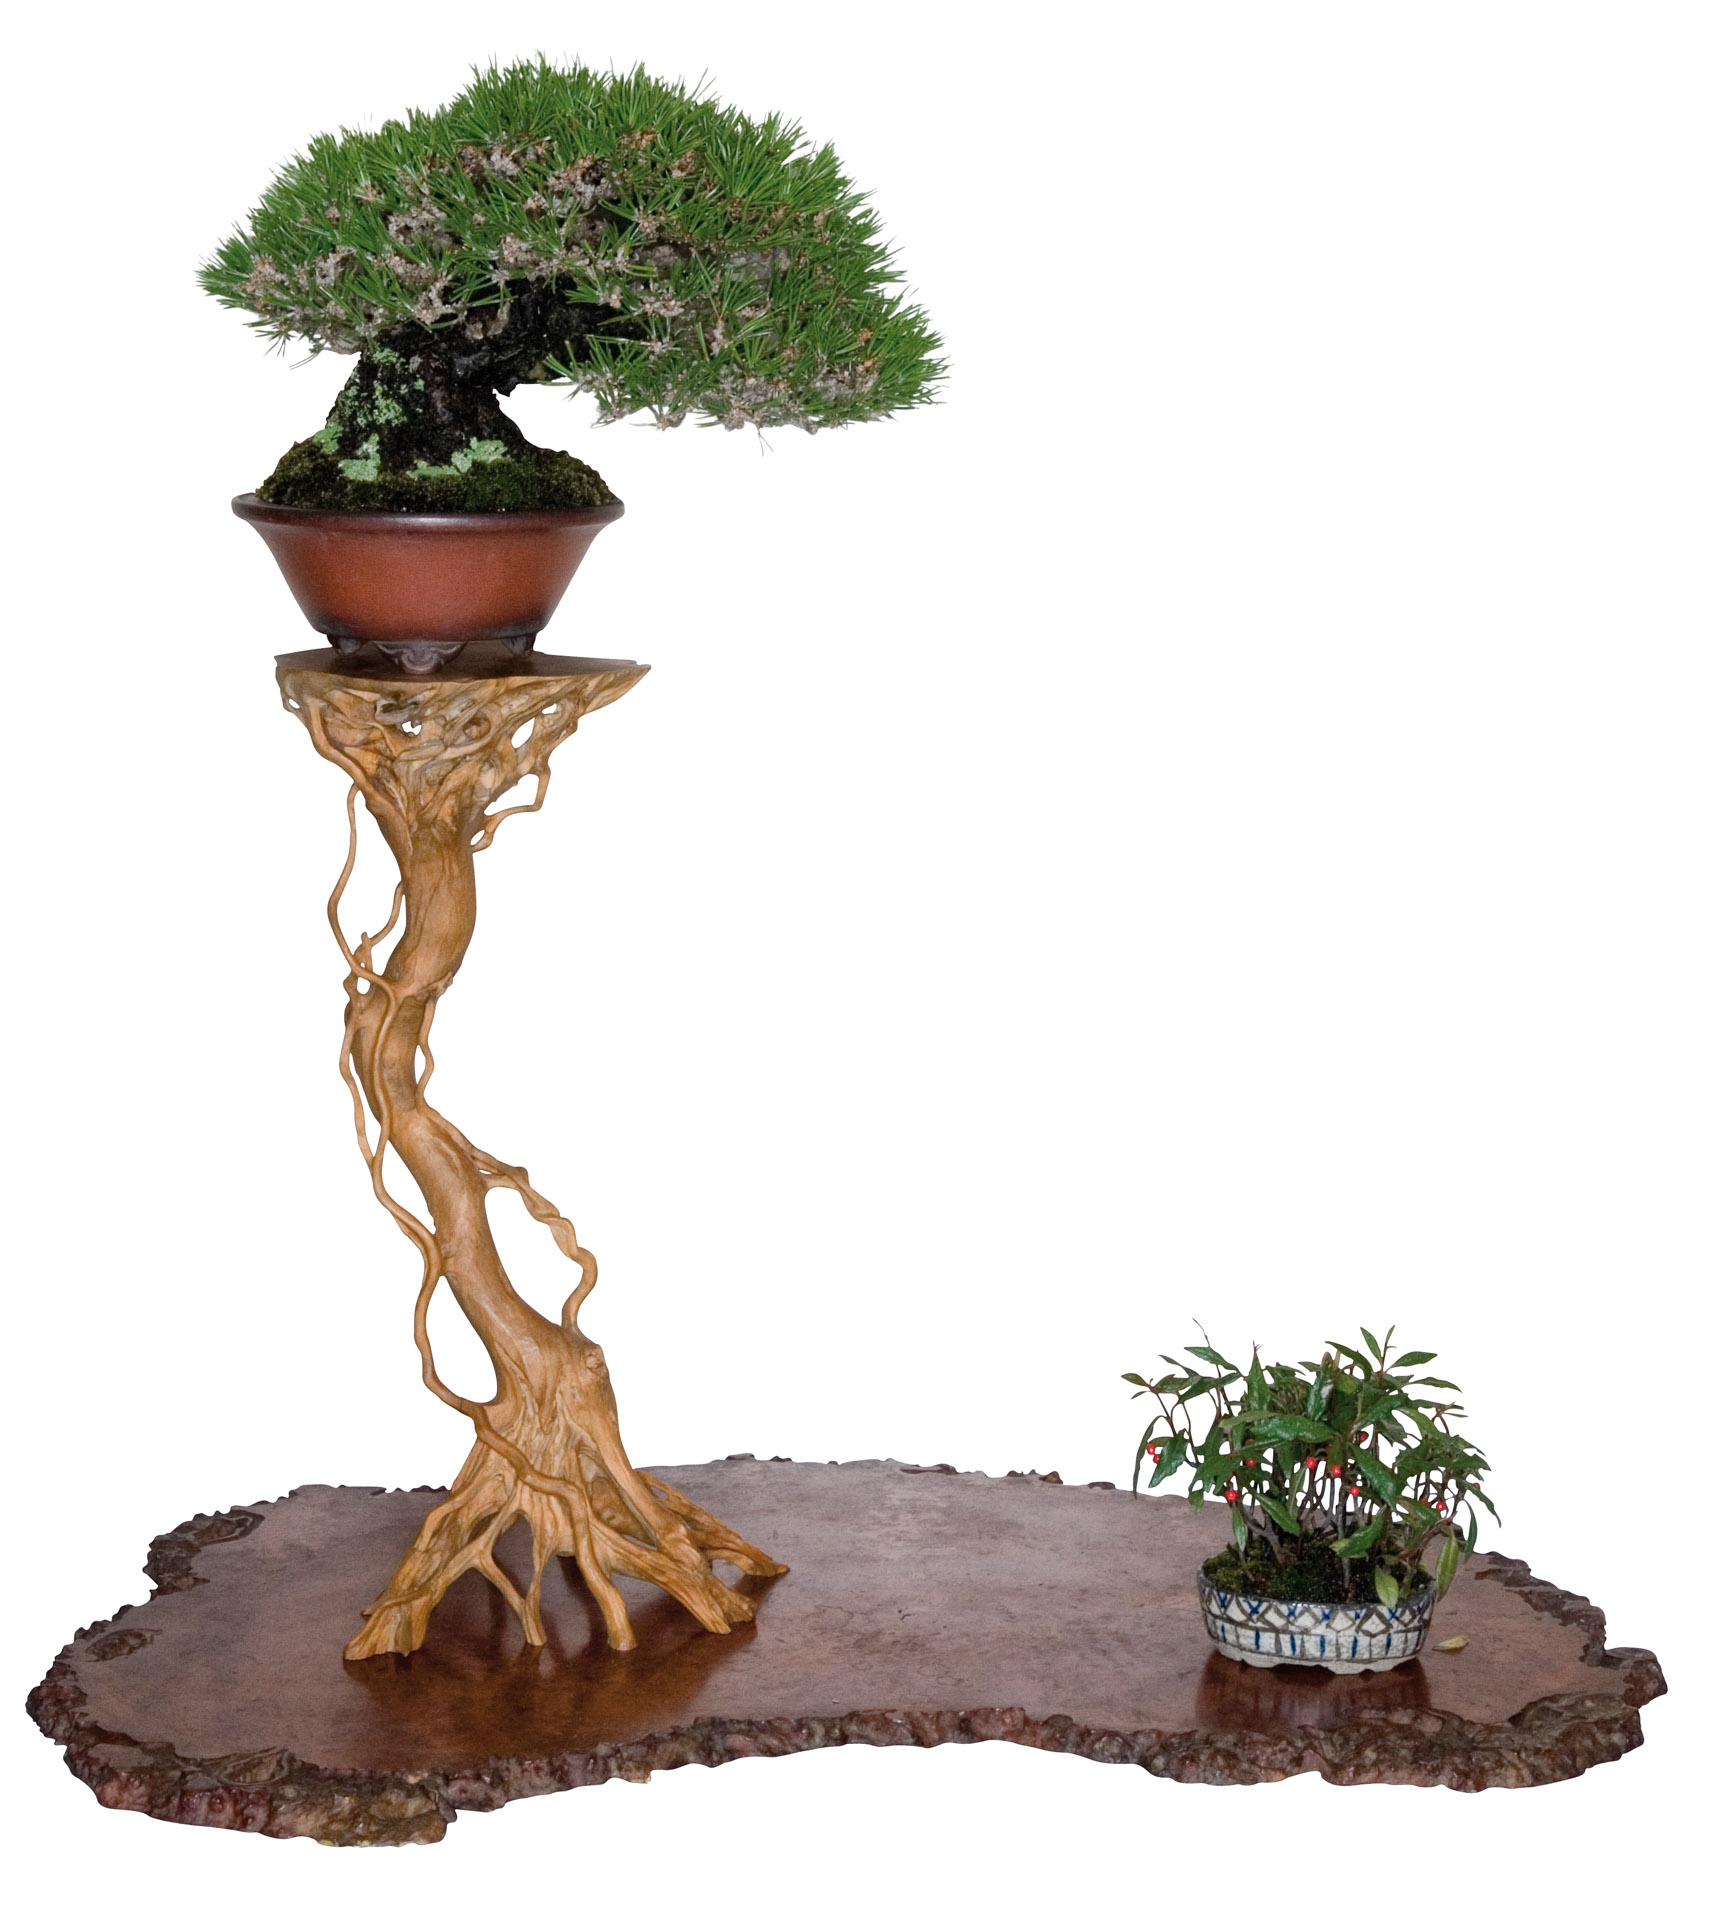
\includegraphics[width=1.0\columnwidth]{2025_05/res/root_stand_display_alt.jpg},\centerline{\emph{A root stand can \textbf{really elevate} a bonsai display.}}]
\end{window}

Before picking up any tools, though, safety comes first! Here's Adam's essential list of \textbf{PPE}:

\begin{itemize}
    \item \textbf{Goggles} --- Protect your eyes from dust and wood chips.
    
    \item \textbf{Mask} --- Essential to avoid inhaling fine dust.
    
    \item \textbf{Cut\--resistant gloves} --- Especially important when using sharp tools.
    
    \item \textbf{Leather apron} --- Adds another layer of protection.
    
    \item \textbf{Thick jumper and double trousers} --- Particularly if you're using powerful tools like a Terrier carver.
\end{itemize}

As Adam put it during the demo: \textit{``You might feel like you're suiting up for battle --- and honestly, that's not far from the truth!''}

\medskip
\topic{The Step\--by\--Step Root Stand Creation Process}
\noindent
Once you're kitted out and ready, it's time for the creative fun to begin. Adam broke down the process into clear, easy\--to\--follow stages:

\begin{itemize}
    \item \textbf{Step 1.} \textit{Level the Log}
    \begin{itemize}
        \item Trim the top and bottom so they're parallel. You want the stand to sit straight and stable.
    \end{itemize}

    \item \textbf{Step 2.} \textit{Sketch the Basic Shape}
    \begin{itemize}
        \item Rough out your stand's silhouette. There's no \textit{``perfect''} way --- go with what the wood suggests.
    \end{itemize}

    \columnbreak

    \item \textbf{Step 3.} \textit{Start Carving the Perforations}
    \begin{itemize}
        \item Using a Dremel, drill, or angle grinder, begin carving holes through the body.
                
        \item Focus on randomness and natural flow.
    \end{itemize}

    Adam stressed: \textit{``Avoid making a neat zigzag pattern --- it'll look man\--made! Think organic, like twisted roots or skull faces.''} 

    \item \textbf{Step 4.} \textit{Refine with Speciality Bits}
    \begin{itemize}
        \item Use \textbf{Terrier bits}, \textbf{ball carving bits}, and \textbf{round nose bits} to smooth and sculpt the form.
        
        \item Create areas of \textit{``negative space''} without sacrificing strength --- especially important for taller, leggier stands.
    \end{itemize}

    \item \textbf{Step 5.} \textit{Sanding}
    \begin{itemize}
        \item Begin sanding with a rotary tool and sanding drums (easier than hand sanding).
        
        \item Start with coarse grits (around 80 grit) to clean up tool marks.
    \end{itemize}

    \item \textbf{Step 6.} \textit{Staining}
    \begin{itemize}
        \item Apply a \textbf{water\--based stain} in your preferred colour.
        
        \item Adam likes to mix his own stains to achieve exactly the tone he wants.
        
        \item Once stained, go over the stand lightly with a stone grinding bit to add texture.
    \end{itemize}

    \item \textbf{Step 7.} \textit{Final Sanding and Finishing}
    \begin{itemize}
        \item Sand the top of the stand progressively finer --- up to 240 grit for most people (or 1500 grit if you're feeling \textit{``extra''}, as Adam joked).
        
        \item Finally, apply your finish of choice:
        \begin{itemize}
            \item[\tiny$\blacksquare$] Danish oil
            \item[\tiny$\blacksquare$] Boiled linseed oil
            \item[\tiny$\blacksquare$] Orange oil
            \item[\tiny$\blacksquare$] Beeswax
            \item[\tiny$\blacksquare$] Polyurethane
            \item[\tiny$\blacksquare$] Varnish
        \end{itemize}
        
        \item Let it dry thoroughly, and your root stand is complete!
    \end{itemize}
\end{itemize}

\medskip
\topic{Tips and Tricks from Adam}
\noindent
Throughout the workshop, Adam shared loads of great practical advice, including:

\begin{itemize}
    \item \textbf{Use the Wood's Natural Features} --- Old branch stubs, knots, or even slight curves can add real character.

    \item \textbf{Avoid Symmetry} --- Nature rarely makes perfect patterns. Let your hand wander a little as you carve.

    \item \textbf{Negative Space is Your Friend} --- Especially for taller stands, more perforations \textit{equals} more elegance (but don't weaken the structure too much!).

    \item \textbf{Finish Smoothly, but Not Too Smoothly} --- Leave a little texture for a more organic feel; perfect glassy finishes can sometimes look artificial.
\end{itemize}

As Adam summed up: \textit{``There's no right or wrong way --- but if it looks like it was made by a machine, you're doing it wrong!''}

\begin{center}
    $\cdots$
\end{center}

\noindent
We hope this guide inspires you to try your hand at carving a bonsai root stand! Whether you make something rough and rustic or polished and intricate, the process itself is incredibly rewarding.  
%
If you have questions, need advice on tools or just fancy trying yourself, don't hesitate to reach out to Adam on WhatsApp to join the next course he is going to organise.

Remember: just like a bonsai, a root stand grows from imagination, patience, and a few happy accidents. See you at the next workshop!

\closearticle
\columnbreak
